\chapter{Praktische Umsetzung und Ergebnisse}
	Im folgenden Abschnitt werden die Durchführung der Studie sowie die genaueren Ergebnisse und Beobachtungen aufgeführt, welche im Verlauf der Studie gewonnen werden konnten. Es werden jedoch nur die reinen Beobachtungen und Ergebnisse hier aufgeführt, die Fazite werden erst in einem späteren Kapitel behandelt.
	\gls{report}
\section{Teilnehmerübersicht}
	Es folgt ein kurzer Überblick über die acht Teilnehmer der Studie.\\
	Insgesamt nahmen acht Kinder an den Terminen teil. Die Kinder waren zum Zeitpunkt dieser Arbeit noch in der Grundschule, jedoch nicht alle in der gleichen Klassenstufe. Die Kinder kannten sich zum Teil bereits untereinander bevor die Studie begann.Es wurde folgende Anzahl von Persönlichkeitstypen im Vorfeld abgegeben: drei Elefanten, zwei Border Collie, zwei Erdmännchen und ein Panda. Die Zuordnung der Tiere lautete wie folgt: Heinz, Lulu und Moritz als Elefanten, Jonas und Mario als Border Collies, Henriette und Benny als Erdmännchen und Sara als Panda.\\
	
	\begin{table}[htbp!]
		\centering
		\begin{tabular}{|
				>{\columncolor[HTML]{C0C0C0}}c |c|c|c|}
			\hline
			\textbf{Typ} & \cellcolor[HTML]{C0C0C0}\textbf{Anzahl n} & \cellcolor[HTML]{C0C0C0}\textbf{Verteilung in \%} & \cellcolor[HTML]{C0C0C0}\textbf{Differenz in \%} \\ \hline
			ENTJ//INFJ   & 2                                         & 25                                                & +2,7                                             \\ \hline
			ENFJ//ESFJ   & 3                                         & 37,5                                              & -27,5                                            \\ \hline
			ISFP//INFP   & 2                                         & 25                                                & -16,4                                            \\ \hline
			INTJ//INFJ   & 1                                         & 12,5                                              & -5.7                                             \\ \hline
		\end{tabular}
		\begin{tabular}{|
				>{\columncolor[HTML]{C0C0C0}}c |c|c|c|}
			\hline
			\textbf{Typ} & \cellcolor[HTML]{C0C0C0}\textbf{Anzahl n} & \cellcolor[HTML]{C0C0C0}\textbf{Verteilung in \%} & \cellcolor[HTML]{C0C0C0}\textbf{Differenz in \%} \\ \hline
				E            & 5                                         & 62,5                                             & +1,0                                                 \\ \hline
				I            & 3                                         & 37,5                                             & -1,0                                                 \\ \hline
				T            & 3                                         & 33,3                                             & -28,5                                                \\ \hline
				F            & 6                                         & 66,6                                             & +28,5                                                \\ \hline
				S            & 5                                         & 62,5                                             & +4,6                                                 \\ \hline
				N            & 3                                         & 37,5                                             & -4,6                                                 \\ \hline
				J            & 6                                         & 75,0                                             & +23,8                                                \\ \hline
				P            & 2                                         & 25,0                                             & -23,8                                                \\ \hline
			\end{tabular}
		\caption[Verteilung der Typen unter den Teilnehmern]{Verteilung der Typen unter den Teilnehmern und Abweichung von Myers und Myers \cite[31]{myers_myers_2002}}
		\label{tab:distribution_type}
	\end{table}
	
	Die Tabelle \ref{tab:distribution_type} zeigt die Verteilung\footnote{Durch das Zusammenfassen von zweier Typen im Test kommen die Buchstaben T und F zusammen häufiger vor als es Teilnehmer gibt} der verschiedenen Persönlichkeitstypen in der oben genannten Gruppe der teilnehmenden Kinder. Dies sollte mit der Abbildung \ref{img:mbti_distribution} verglichen werden. Die Zahlen decken sich in manchen Fällen mit den Werten, welche von Myers-Briggs ermittelt wurden \cite[31]{myers_myers_2002}. Jedoch in den meisten Fällen liegen die Werte, die die Teilnehmer der Studie lieferten, deutlich neben den Werten von Myers-Briggs. Dies kann verschiedene Ursachen haben. Erstens, der Test ist auf Englisch, welches die Kenntnisse der Kinder übersteigt und deshalb die Eltern der Kinder helfen müssen und so unter Umständen verfälschte Werte herauskommen können. Zweitens, die Anzahl der Probanden, die diesen Test durchgeführt und die Werte übermittelt haben, liegen deutlich unter der Anzahl, die für Abbildung \ref{img:mbti_distribution} verwendet wurde. Daher ist eine größere Abweichung bei den Werten der Autoren dieser Arbeit nicht ungewöhnlich.
\section{Durchführung}
	Vor Beginn der Studie führten alle Teilnehmer einen Persönlichkeitstest durch, der jedes der teilnehmenden Kinder einem Tier zuordnete. Der Test besteht aus 38 verschiedenen Fragen, jede dieser Frage bietet zwei Antwortmöglichkeiten. Am Ende dieses Tests bekommt der Teilnehmer als Ergebnis ein Tier entweder aus der Kategorie der extrovertierten oder der introvertierten Persönlichkeitstypen (vgl. Abbildung \ref{img:animals}). 
	\begin{figure}[htbp!]
		\centering
		\fbox{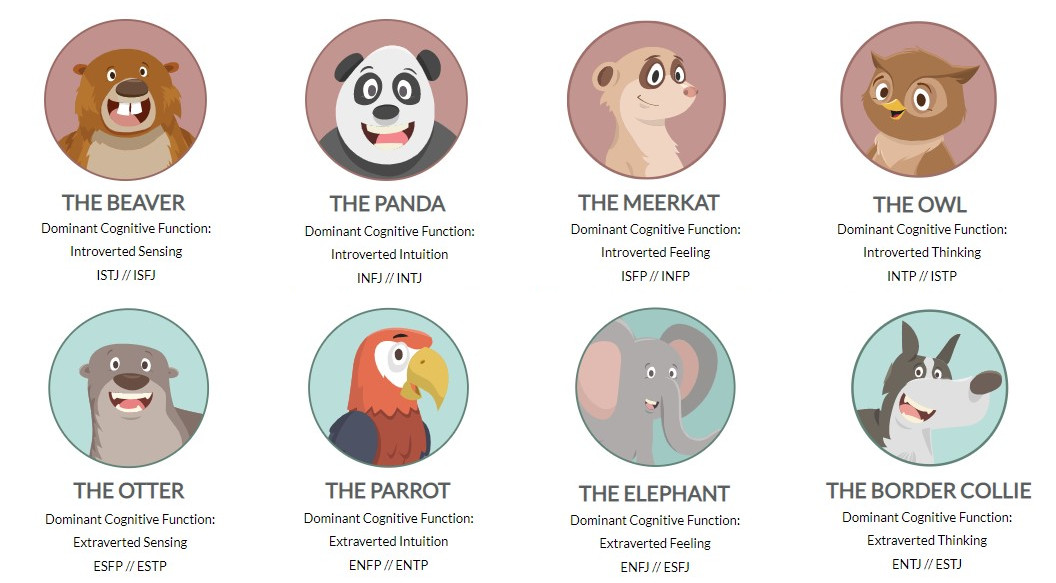
\includegraphics[width=0.4\textheight,angle=0]{img/animals}}
		\caption[Alle Tiere des Persönlichkeitstests]{Alle Tiere des Persönlichkeitstests \cite{knowAndLove}}
		\label{img:animals}
	\end{figure} 
	In der ersten Stunde der Studie mussten alle Teilnehmer den Computational Thinking Test durchführen. Die Auswertung der Ergebnisse aus der ersten Stunde jedes Teilnehmers befinden sich in Tabelle \ref{tab:data}. Wie bereits erwähnt, besteht dieser Test aus mehreren Kategorien, die normalisierten Ergebnisse befinden sich in Abbildung \ref{img:auswertung}.\\
	Die Termine der Studie können in zwei Phasen eingeteilt werden. Die erste Phase ist die Phase, in der die Kinder sich mit Lego WeDo vertraut machten. Die jeweiligen Termine hatten ein eigenes Thema, welches von der WeDo-App angeboten wurde. Die Autoren stellten zu Beginn eines Termins den Kindern Fragen zum Thema und es wurde über das Thema diskutiert. Nachdem die Diskussionsrunde vorbei war, führten die Kinder selbständig die von der WeDo-App bereitgestellten Kurse zu dem Thema durch während die Autoren die Kinder beobachteten und dabei Notizen in einem Fragebogen machten. Der Fragebogen wird im weiteren Verlauf noch genauer erklärt. Die zweite Phase läutete den Beginn des Wettbewerbs ein. Die beiden Gruppen, je vier Teilnehmer, erhielten ein sogenanntes Motivationsset von Lego, welches zusätzlich zu den bis dahin verwendeten Kästen verwendet wurden. Der Aufbau dieser Termine ähnelte dem von Phase eins: Jeder Teilnehmer bekam mit dem Motivationsset ein sogenanntes IngenieurInnen-Notizbuch (vgl. Abbildung \ref{img:explorer_heft}). In jedem Heft sind Aufgaben für die Kinder, insgesamt existieren 12 dieser Treffen, welche alle auf den Wettbewerb hinführen. Bei jedem dieser Treffen wird ein Thema, wie bereits in Phase eins besprochen, bevor die Kinder anschließend selbständig die weiteren Aufgaben lösten. Auch hier notierten die Autoren das Verhalten der Kinder und trugen dies in den Fragebogen ein.
	\begin{figure}[htbp!]
		\centering
		\fbox{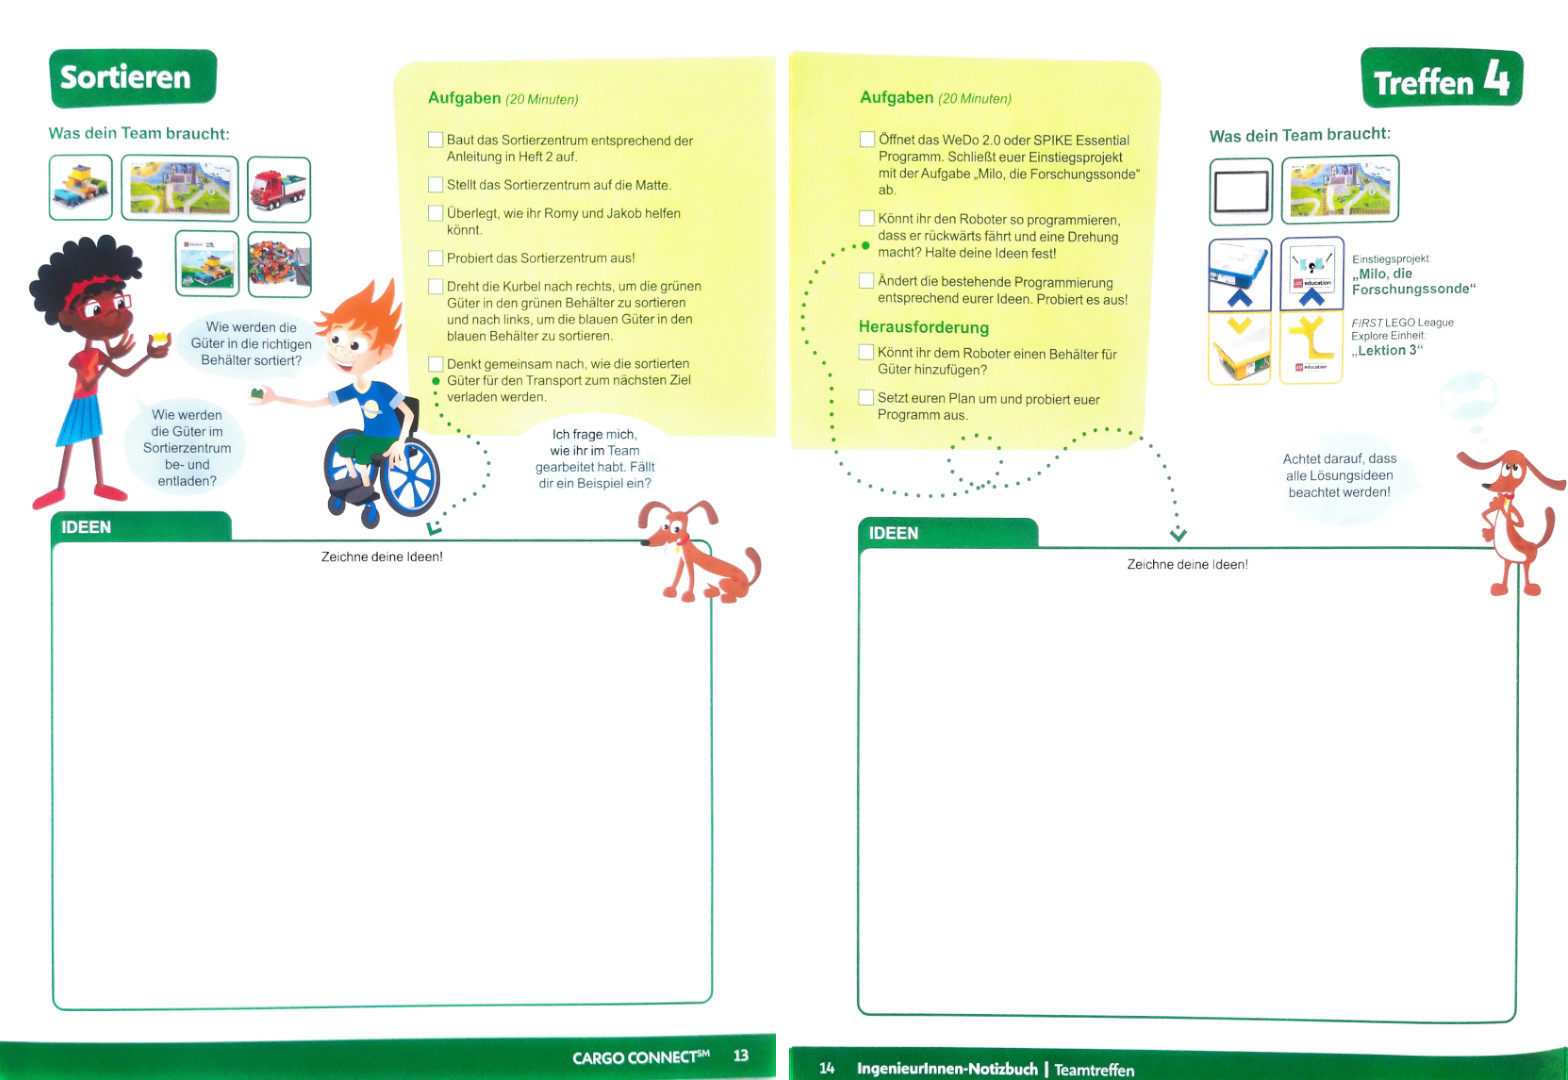
\includegraphics[width=0.3\textheight,angle=0]{img/Explorer}}
		\caption[Ausschnitt aus dem IngenierurInnen-Heft]{Ausschnitt aus dem IngenierurInnen-Heft}
		\label{img:explorer_heft}
	\end{figure}
	
\section{Ergebnisse}
	\subsection{Computational Thinking Test}
	
	\begin{table}[htbp!]
		\centering
		\begin{tabular}{|
				>{\columncolor[HTML]{C0C0C0}}c |c|c|c|c|c|c|c|}
			\hline
			\textbf{Name} &
			\cellcolor[HTML]{C0C0C0}\textbf{Typ 1} &
			\cellcolor[HTML]{C0C0C0}\textbf{Typ 2} &
			\cellcolor[HTML]{C0C0C0}\textbf{Typ 3} &
			\cellcolor[HTML]{C0C0C0}\textbf{Typ 4} &
			\cellcolor[HTML]{C0C0C0}\textbf{Typ 5} &
			\cellcolor[HTML]{C0C0C0}\textbf{Typ 6} &
			\cellcolor[HTML]{C0C0C0}\textbf{Total} \\ \hline
			
		
			Henriette            & 6 & 5 & 7 & 2 & 2 & 3 & 25 \\ \hline
			Moritz               & 6 & 5 & 7 & 2 & 2 & 3 & 25 \\ \hline
			Heinz                & 6 & 5 & 7 & 2 & 1 & 3 & 24 \\ \hline
			Benny                & 6 & 5 & 7 & 2 & 0 & 3 & 23 \\ \hline
			Lulu                 & 6 & 4 & 6 & 2 & 2 & 3 & 23 \\ \hline	
			Mario                & 6 & 4 & 3 & 2 & 1 & 2 & 17 \\ \hline
			Sara                 & 6 & 2 & 7 & 0 & 1 & 1 & 17 \\ \hline		
			Jonas                & 0 & 2 & 3 & 1 & 1 & 3 & 10 \\ \hline
			\textbf{Maximalwert} & 6 & 5 & 7 & 2 & 2 & 3 & 25 \\ \hline
		\end{tabular}
		\caption{Erreichte Punkte pro Kategorie}
		\label{tab:data}
	\end{table}
	
	In der obenstehenden Tabellen sind die Anzahl der Punkte aufgeführt, die die einzelnen Teilnehmer, hier mit Pseudonym aufgeführt, erreicht haben. Wie aus der letzten Zeile deutlich wird, sind unterschiedliche Maximalpunkte erreichbar. Daher wurden für die beiden folgenden Abbildungen die Werte dieser Tabelle auf 10 normalisiert. Dabei ist zu sehen, dass besonders in Kategorie 1, welche reine Sequenzen abfragte, und Kategorie 3, die den Umgang mit verschachtelten Schleifen prüfte, fast alle Probanden außer Jonas die volle Punktzahl erreicht haben, da er die Fragen nicht eindeutig beantwortet hatte und deshalb ihm keine Punkte gegeben werden konnte.	\\ 
	
	
	\begin{figure}[htbp!]
		\centering
		\begin{tikzpicture}
			\tkzKiviatDiagram[scale=.5,label distance=.5cm,
			radial  = 5,
			gap     = 1,  
			lattice = 10]{Typ 1,Typ 2,Typ 3,Typ 4 ,Typ 5, Typ 6}
			%Jonathan
			\tkzKiviatLine[thick,color=blue,mark=none!20,opacity=1](10,8,4.285714286,10,5,6.666666667)
			%Annabell
			\tkzKiviatLine[thick,color=green,mark=none!20,opacity=.85](10,10,10,10,10,10)
			%Luise
			\tkzKiviatLine[thick,color=yellow,mark=none!20,opacity=.5](10,8,8.571428571,10,10,10)
			%Benny
			\tkzKiviatLine[thick,color=magenta,mark=none!20,opacity=.85](8.333333333,6,4.285714286,5,0,3.333333333)
			%Mohammed
			\tkzKiviatLine[thick,color=orange,mark=none!20,opacity=.85](10,10,10,10,5,10)
			%Yufei
			\tkzKiviatLine[thick,color=brown,mark=none!20,opacity=.85](10,4,10,0,5,3.333333333)
			%Henrik
			\tkzKiviatLine[thick,color=purple,mark=none!20,opacity=.85](0,4,4.285714286,5,5,10)
			%Namenslos
			\tkzKiviatLine[thick,color=teal,mark=none!20,opacity=.85](10,10,10,10,10,10)
			%Maximalwert
			%\tkzKiviatLine[thick,color=black,mark=none,
			%fill=black!20,opacity=1](10,10,10,10,10,10)
			\tkzKiviatGrad[prefix=,unity=1](1)  
			
		\end{tikzpicture}
		\caption[Auswertung]{Auswertung der Tests}
		\label{img:auswertung}
	\end{figure}
	
	Abbildung \ref{img:auswertung} verwendet die normalisierten Werte aus Tablle \ref{tab:data}. Sichtbar wird hier besonders der Einbruch in der Kategorie für Bedingungen mit If und Else, nur ein Proband konnte hier alle Fragen richtig beantworten. Bei Kategorie 3 ist erkennbar, dass es hier wohl große Unterschiede zwischen den einzelnen Teilnehmern gibt, da hier die Extremwerte eine Differenz von etwas unter 6 Punkten, also fast 60\% Unterschied sichtbar wird. Auch die Typen 2 und 6 weisen ähnliche Muster auf, wobei bei Typ 6 die Differenz über 6 liegt. Typ 1 und Typ 4 dagegen ist bei allen Teilnehmern fast gleich gut, hier ist die Differenz der Extremen deutlich geringer.\\ 
	
	
	
	
	
	\begin{figure}[htbp!]
		\centering
		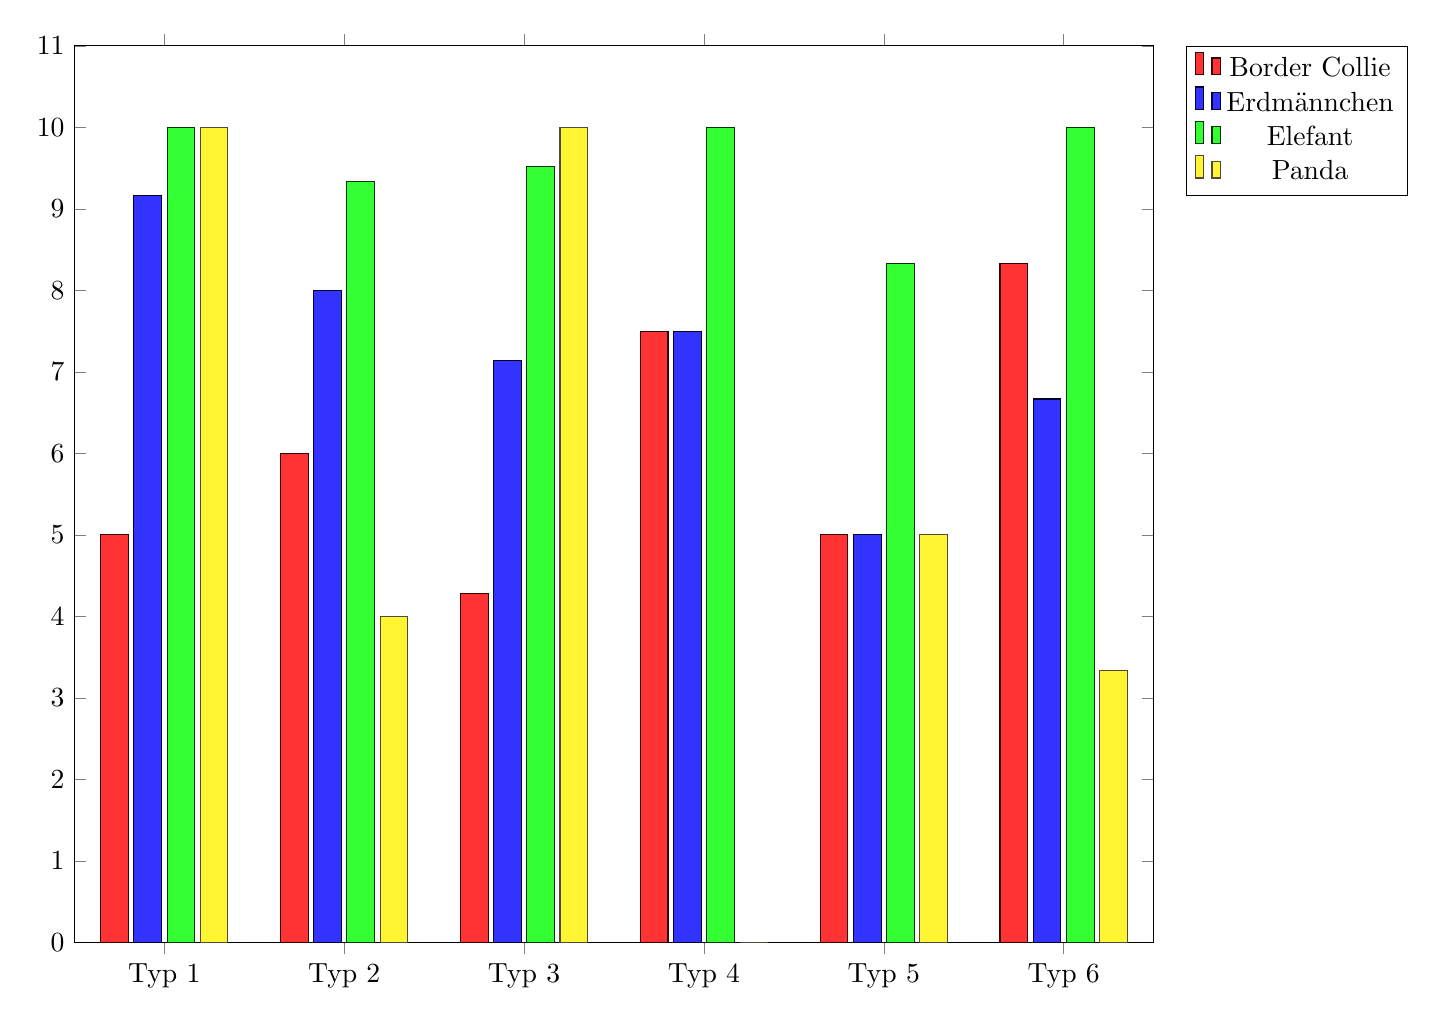
\begin{tikzpicture}
			\begin{axis}[
				ybar,ymin=0,
				symbolic x coords={Typ 1, Typ 2, Typ 3, Typ 4, Typ 5, Typ 6},xtick={Typ 1, Typ 2, Typ 3, Typ 4, Typ 5, Typ 6 
				}, scale = 2,legend pos=outer north east
				]
				%Border Collie
				\addplot[red!20!black,fill=red!80!white] coordinates
				{(Typ 1,5) (Typ 2,6) (Typ 3,4.285714286) (Typ 4,7.5) (Typ 5,5) (Typ 6,8.333333333)};
				%Erdmännchen 9,166666667	8	7,142857143	7,5	5	6,666666667
				\addplot[blue!20!black,fill=blue!80!white] coordinates
				{(Typ 1,9.16666667) (Typ 2,8) (Typ 3,7.142857143) (Typ 4,7.5) (Typ 5,5) (Typ 6,6.66666667)};
				%Elefant
				\addplot[green!20!black,fill=green!80!white] coordinates
				{(Typ 1,10) (Typ 2,9.333333333) (Typ 3,9.523809524) (Typ 4,10) (Typ 5,8.333333333) (Typ 6,10)};
				%Panda
				\addplot[yellow!20!black,fill=yellow!80!white] coordinates
				{(Typ 1,10) (Typ 2,4) (Typ 3,10) (Typ 4,0) (Typ 5,5) (Typ 6,3.33333333)};
				\addlegendentry{Border Collie}
				\addlegendentry{Erdmännchen}
				\addlegendentry{Elefant}
				\addlegendentry{Panda}
			\end{axis}
		\end{tikzpicture}
		\caption[Auswertung Durchschnitt]{Durchschn. Punkte pro Kategorie der einzelnen Typen, normalisiert}
		\label{img:auswertung_typus}
	\end{figure}

	Ebenfalls die normalisierten Werte verwendet auch Abbildung \ref{img:auswertung_typus}. Hierbei wird der Durchschnitt der einzelnen Typen pro Kategorie des Tests dargestellt. Auffallend ist besonders der Typ Border Collie und Elefant. Border Collie hat eine relativ geringe Durchschnittspunktzahl in den Testkategorien erreicht, Elefant dagegen erreichte in der Hälfte aller Kategorien den Maximalwert, in der anderen Hälfte kam dieser Typ nahe ans Maximum. Der Panda dagegen hat eine relativ hohe Streuung, die Werte liegen im kompletten Bereich von 0 bis inklusive 10.\\

\section{Beobachtungen}
	\subsection{Der Fragebogen}
	
	\subsection{Empirische Beobachtungen}
	Die Gruppe der zwei Erdmännchen und zwei der drei Elefanten startete mit viel guter Kommunikation und gutem Teamwork in das Projekt. Die Aufgaben wurden meist schnell und gut gelöst, manchmal drängten die Kinder zu noch mehr und hatten einen großen Verbesserungsdrang.\\
	Die Gruppe aus Panda, Elefant und zwei Border Collies hatte große Startschwierigkeiten, die Kommunikation zwischen den einzelnen Kindern funktionierte nur sehr schlecht, kamen kaum voran und hatten als große Gruppe Schwierigkeiten, die Aufgaben zu lösen. Bei dieser Gruppe traten auch vermehrt Schwierigkeiten im Vergleich zur ersten Gruppe bei der Lösung für den Computational Thinking Test auf.
	Trotz allem wurden am Ende die Aufgaben von den Gruppen gelöst, wenn vereinzelt Fehler auftraten wurden diese auch schnell gelöst. Das liegt allerdings auch daran, dass die Programme, die zu programmieren waren, bereits vorgegeben waren. Die Fehler, die dann auftraten, waren Fehler, deren Lösung man den Kindern noch nicht zutrauen kann.\\
	Bei Besprechungen, sowohl zu Beginn als auch gegen Ende der Termine, dominierte Benny (Erdmännchen) und Moritz (Elefant). Einzelne Beiträge kamen auch durch die anderen Teilnehmer, meistens waren jedoch die beiden genannten Teilnehmer die ersten die sich meldeten, einige Male auch die einzigen. Die Beiden waren in der Lage, besser allein zu arbeiten als im Team, konnten trotzdem auch im Team gut mitarbeiten.
	In Zweiergruppen war die Kommunikation zwischen den einzelnen Kindern bei allen Gruppen ungefähr gleich gut, Anweisungen wurden befolgt und konnten auch gut formuliert werden. Ergebnisse wurden nach wie vor von allen Gruppen geliefert, mal schneller und mal langsamer. Teilweise waren die Teilnehmer auch in der Lage, ihre Bauten vorzustellen und zu erklären. Besonders Mario (Border Collie) fragte bereits während der Bauphasen nach Feedback, ein Verhalten, das bei keinem anderen Teilnehmer dokumentiert werden konnte.\\ 
	In der Endphase der genannten Termine wurde eine Verschiebung der Qualität der Kommunikation der Gruppen bemerkbar. Die zu Beginn starke Gruppe um Benny mit Lulu, Henriette und Moritz, aufgeteilt in Zweiergruppen, konnte gar nicht mehr zusammenarbeiten, aus Arbeiten wurde viel Reden über verschiedene Dinge bis hin zu kleineren Streitereien über Bauteile. Bei der anderen Gruppe dagegen wurde es deutlich besser, das Zusammenarbeiten funktionierte sehr gut und am Ende konnten auch gute Ergebnisse vorgestellt werden. Die erste Gruppe konnte die Ergebnisse aufgrund von Zeitgründen oftmals nicht präsentieren.\\
	In den meisten Fällen wurden alle von allen gleichbehandelt, in einzelnen Fällen trat die Dominanz von Moritz und Benny hervor. Besonders am Anfang trat dies häufiger auf. Ein paar Kinder zeigten fantastisches Denken auf. Grundverständnis für algorithmisches Denken war da. Muster wurden selten erwähnt, Gelerntes wurde aber wieder angewandt. Ein nennenswertes Abstraktionsverhalten konnte nicht wirklich beobachtet werden.